\documentclass[a4paper,10pt]{article}

\usepackage{PRIMEarxiv}
\usepackage[utf8]{inputenc}
\usepackage[T1]{fontenc}
\usepackage{amsmath,amssymb,amsfonts}
\usepackage{booktabs}
\usepackage{graphicx}
\usepackage{tabularx}
\usepackage{array}
\usepackage{multirow}
\usepackage{setspace}
\usepackage{xcolor}
\usepackage{fancyhdr}
\usepackage{hyperref}
\usepackage{url}
\usepackage{microtype}
\usepackage{tikz}
\usepackage{float}
\usepackage[section]{placeins}
\usepackage{needspace}
\usetikzlibrary{arrows.meta,positioning,calc,fit}

\geometry{a4paper}
\AtBeginDocument{\newgeometry{top=2.5cm,bottom=2.5cm,left=2.5cm,right=2.5cm,headheight=14pt,headsep=18pt,footskip=25pt}}
\onehalfspacing
\emergencystretch=1.5em

\pagestyle{fancy}
\fancyhf{}
\fancyhead[L]{\textit{Course-Aligned Polyp Segmentation Ablation}}
\cfoot{\thepage}
\renewcommand{\headrulewidth}{0pt}

\hypersetup{colorlinks=true,linkcolor=black,citecolor=black,urlcolor=blue,hypertexnames=false}
\newcolumntype{Y}{>{\raggedright\arraybackslash}X}
% Placeholder values. Run python run_all_experiments.py to replace these.
\newcommand{\BestModelName}{TBD}
\newcommand{\BestDice}{TBD}
\newcommand{\BestIoU}{TBD}
\newcommand{\DiceGain}{TBD}
\newcommand{\HardwareName}{TBD}
\newcommand{\TorchVersion}{TBD}
\newcommand{\CudaVersion}{TBD}
\newcommand{\UNetDice}{TBD}
\newcommand{\UNetIoU}{TBD}
\newcommand{\UNetPrecision}{TBD}
\newcommand{\UNetRecall}{TBD}
\newcommand{\UNetHD}{TBD}
\newcommand{\UNetParams}{TBD}
\newcommand{\UNetLatency}{TBD}
\newcommand{\AttentionUNetDice}{TBD}
\newcommand{\AttentionUNetIoU}{TBD}
\newcommand{\AttentionUNetPrecision}{TBD}
\newcommand{\AttentionUNetRecall}{TBD}
\newcommand{\AttentionUNetHD}{TBD}
\newcommand{\AttentionUNetParams}{TBD}
\newcommand{\AttentionUNetLatency}{TBD}
\newcommand{\TransformerUNetDice}{TBD}
\newcommand{\TransformerUNetIoU}{TBD}
\newcommand{\TransformerUNetPrecision}{TBD}
\newcommand{\TransformerUNetRecall}{TBD}
\newcommand{\TransformerUNetHD}{TBD}
\newcommand{\TransformerUNetParams}{TBD}
\newcommand{\TransformerUNetLatency}{TBD}
\newcommand{\ProposedDice}{TBD}
\newcommand{\ProposedIoU}{TBD}
\newcommand{\ProposedPrecision}{TBD}
\newcommand{\ProposedRecall}{TBD}
\newcommand{\ProposedHD}{TBD}
\newcommand{\ProposedParams}{TBD}
\newcommand{\ProposedLatency}{TBD}


\tikzset{
  block/.style={draw,rounded corners,thick,align=center,minimum height=8mm,text width=20mm,fill=blue!8},
  enc/.style={block,fill=green!10},
  dec/.style={block,fill=orange!12},
  att/.style={draw,rounded corners,thick,align=center,minimum height=7mm,text width=16mm,fill=yellow!18},
  trans/.style={draw,rounded corners,very thick,align=center,minimum height=10mm,text width=30mm,fill=violet!12},
  flow/.style={-{Latex[length=2mm]},thick},
  skip/.style={-{Latex[length=2mm]},thick,dashed}
}

\title{Structural and Visual Intelligence for Colonoscopy Polyp Segmentation:\\
A Controlled Ablation of Attention Gates and a Lightweight Transformer Bottleneck on Kvasir-SEG}

\author{
Oussama Hammir \\
Student ID: 25sf51073 \\
School of Computer Science and Technology \\
Harbin Institute of Technology, Shenzhen, China \\
Advanced Artificial Intelligence Course Lab \\
\href{mailto:hammiroussama@gmail.com}{\texttt{hammiroussama@gmail.com}} \\
Supervisor: Luyao
}

\begin{document}
\maketitle
\thispagestyle{empty}

\begin{abstract}
Colonoscopy polyp segmentation is a visual-intelligence task in which every image pixel is classified as polyp or background. The task is difficult because polyps vary in scale, morphology, illumination, texture, and boundary contrast. Following the Advanced Artificial Intelligence course framework, this study connects structural intelligence through convolutional encoder--decoder networks, visual intelligence through dense semantic segmentation, and language-intelligence-derived self-attention through a lightweight Transformer bottleneck. Two modifications to a standard U-Net are evaluated: attention-gated skip connections and bottleneck self-attention. Four configurations are trained on Kvasir-SEG under one controlled protocol: U-Net, Attention U-Net, Transformer U-Net, and a combined attention-plus-Transformer model. The experiment uses a deterministic 70/15/15 train--validation--test split, $256\times256$ inputs, BCE--Dice loss, AdamW, seed 42, early stopping, and identical augmentation. Evaluation includes Dice, Intersection over Union (IoU), precision, recall, 95th-percentile Hausdorff distance (HD95), parameter count, and inference latency. Transformer U-Net achieved the best overall result, with Dice \BestDice, IoU \BestIoU, precision \TransformerUNetPrecision, and HD95 \TransformerUNetHD~pixels. It improved Dice over U-Net by \DiceGain~and reduced HD95 by approximately 40.8\%. The combined model obtained the highest recall (\ProposedRecall) but did not improve Dice or IoU and increased latency to \ProposedLatency~ms per image. The experiment demonstrates that global context was the most beneficial tested component and that combining individually useful modules does not guarantee additive gains. The complete reproducibility package is available at \url{https://github.com/hammiroussama/lightweight-transformer-unet-kvasir}.
\end{abstract}

\keywords{Visual Intelligence \and Semantic Segmentation \and U-Net \and Transformer \and Kvasir-SEG}

\clearpage
\setcounter{page}{1}

\section{Introduction}
\label{sec:introduction}

A colorectal polyp is an abnormal tissue growth that projects from the intestinal lining. Some polyps can develop toward colorectal cancer, so colonoscopy is used to detect and remove suspicious lesions. Pixel-level segmentation complements detection by estimating the exact polyp region, which can support visualization, size measurement, and computer-aided analysis. The task remains difficult because polyps vary in size, color, texture, morphology, camera distance, and illumination, while their boundaries may be blurred, occluded, or visually similar to surrounding mucosa.

This project is directly connected to the Advanced Artificial Intelligence course knowledge system \cite{hitsz2026aai}. U-Net represents \emph{structural intelligence} through a convolutional encoder--decoder and \emph{visual intelligence} through dense segmentation. Attention gates improve feature selection inside the visual model, while the Transformer bottleneck transfers self-attention, originally developed for sequence and language intelligence, into visual representation learning \cite{vaswani2017attention}. The experiment therefore studies how local convolutional inductive bias, selective skip fusion, and global contextual modeling interact in one practical vision task.

U-Net is a strong medical-segmentation baseline because its contracting path extracts semantic features and its expanding path reconstructs spatial detail through skip connections \cite{ronneberger2015unet}. However, direct skip fusion may transmit irrelevant background responses. Attention U-Net addresses this problem by learning gates that emphasize target-related encoder features \cite{oktay2018attention}. Convolution also models distant relationships only indirectly through repeated local operations, whereas Transformer self-attention directly relates spatially separated tokens. Hybrid architectures such as TransUNet consequently combine convolutional localization with global contextual reasoning \cite{chen2024transunet}.

The central research question is:
\begin{quote}
\emph{Do attention-gated skip connections and a lightweight Transformer bottleneck improve U-Net segmentation on Kvasir-SEG without introducing excessive parameter and inference costs?}
\end{quote}

The main contributions are:
\begin{itemize}
    \item a course-aligned architecture study integrating CNN structural intelligence, visual segmentation, and Transformer self-attention in a controlled $2\times2$ ablation;
    \item a reproducible four-model experiment using an identical split, preprocessing, optimization protocol, checkpoint rule, and multi-dimensional evaluation of accuracy, boundaries, parameters, and latency; and
    \item an evidence-based analysis showing which component contributes most, where the models fail, and why additional architectural complexity does not necessarily yield additive performance.
\end{itemize}

The complete source code is available in the \href{https://github.com/hammiroussama/lightweight-transformer-unet-kvasir}{public GitHub repository}. Section~\ref{sec:related} reviews the research and course foundations, Section~\ref{sec:method} presents the methodology, Section~\ref{sec:experiments} defines the experimental protocol, Section~\ref{sec:results} reports quantitative and visual evidence, and Sections~\ref{sec:discussion} and \ref{sec:conclusion} interpret and conclude the study.

\section{Related Work and Course Foundations}
\label{sec:related}

\subsection{U-Net-Based Medical Segmentation}

U-Net consists of a symmetric encoder-decoder with skip connections between corresponding scales \cite{ronneberger2015unet}. The encoder produces contextual features through convolution and downsampling, while the decoder upsamples and combines semantic representations with spatial detail. This structure is especially suitable for medical tasks with limited annotated data. However, direct concatenation assumes that all encoder responses are useful for reconstruction.

Attention U-Net introduced additive attention gates to condition encoder skips on coarser decoder context \cite{oktay2018attention}. The gates suppress irrelevant activations and highlight features associated with the target. Because the mechanism is inserted into skip pathways, it can improve selectivity with relatively limited overhead. For polyp segmentation, this may help when specular highlights, folds, instruments, or background mucosa create strong but irrelevant local responses.

\subsection{Transformers in Medical Segmentation}

Self-attention maps each token to query, key, and value representations and computes pairwise content-dependent interactions. The standard operation is
\begin{equation}
\operatorname{Attention}(Q,K,V)=\operatorname{Softmax}\left(\frac{QK^{\top}}{\sqrt{d_k}}\right)V.
\end{equation}
Transformers can therefore represent long-range dependencies explicitly, but their quadratic token complexity is expensive at high image resolution. Hybrid models reduce this cost by applying attention after convolutional downsampling. TransUNet is a representative example: convolutional features preserve local information, and a Transformer encoder captures global context before U-shaped decoding \cite{chen2024transunet}. The present method follows the same high-level motivation but uses a substantially smaller bottleneck module and no large pretrained Transformer backbone.

\subsection{Kvasir-SEG}

Kvasir-SEG contains 1,000 gastrointestinal polyp images and corresponding expert-verified masks \cite{jha2020kvasir}. Image resolutions vary, making fixed resizing necessary for batch training. The dataset is appropriate for a course-scale controlled experiment, but its size and single-domain nature limit conclusions about clinical generalization. This study therefore emphasizes internal ablation rather than claims of state-of-the-art performance.

\subsection{Course Correlation and Research Positioning}

The course organizes advanced AI into structural, visual, language, generative, graph, multimodal, reinforcement, and agent intelligence modules \cite{hitsz2026aai}. The present experiment focuses experimentally on three closely related elements: CNN-based structural intelligence, semantic-segmentation visual intelligence, and Transformer self-attention transferred from language intelligence. CNNs provide locality, translation-aware feature extraction, and hierarchical representations \cite{goodfellow2016deep}; self-attention supplies content-dependent global interactions. The study does not claim to implement all eight modules. Instead, it demonstrates cross-module transfer by applying a language-originated mechanism to a visual task and evaluating it against a controlled convolutional baseline.

The research difference from the cited architectures is methodological rather than scale-oriented. It does not claim a new state-of-the-art backbone or reproduce a large pretrained TransUNet. Instead, it enables and tests a $2\times2$ controlled ablation in which attention gates and a compact Transformer bottleneck are independently enabled or disabled while every training condition remains fixed. This design supports the course objective of systematically comparing mainstream AI architectures and identifying when additional modules provide genuine practical value.


\section{Methodology and Proposed Architecture}
\label{sec:method}

\subsection{Problem Formulation}

Given an RGB colonoscopy image $X\in\mathbb{R}^{H\times W\times 3}$ and binary reference mask $Y\in\{0,1\}^{H\times W}$, the model predicts logits $Z=f_{\theta}(X)$. The foreground probability is $P=\sigma(Z)$, and the binary prediction is $\hat{Y}=\mathbb{I}(P\geq 0.5)$.

\subsection{Course Theoretical Preliminaries}

A convolutional feature block maps an input representation $F^{(l-1)}$ to
\begin{equation}
F^{(l)}=\phi\!\left(\operatorname{BN}\!\left(W^{(l)}*F^{(l-1)}+b^{(l)}\right)\right),
\end{equation}
where $*$ denotes convolution, $\operatorname{BN}$ is batch normalization, and $\phi$ is ReLU. The local receptive field and shared weights provide the structural inductive bias used by U-Net. Skip connections preserve high-resolution visual information, while decoder stages combine this detail with deeper semantic context.

The Transformer component treats the bottleneck feature map as a sequence of visual tokens. Multi-head self-attention allows each token to aggregate information from distant locations, complementing convolutional locality. Applying attention only after $16\times$ downsampling keeps the token sequence small and makes the cross-module design computationally feasible for a course-scale experiment.


\subsection{Architecture}

Figure~\ref{fig:architecture} shows the full attention-plus-Transformer variant used in the ablation. Four convolutional encoder stages progressively halve spatial resolution and double feature channels. At the deepest level, a depthwise convolution supplies spatial positional bias and a compact Transformer encoder processes flattened bottleneck tokens. The decoder then upsamples features through transposed convolution. Before each skip is concatenated, an additive attention gate uses the current decoder feature as a gating signal.

\begin{figure}[H]
\centering
\resizebox{0.94\textwidth}{!}{%
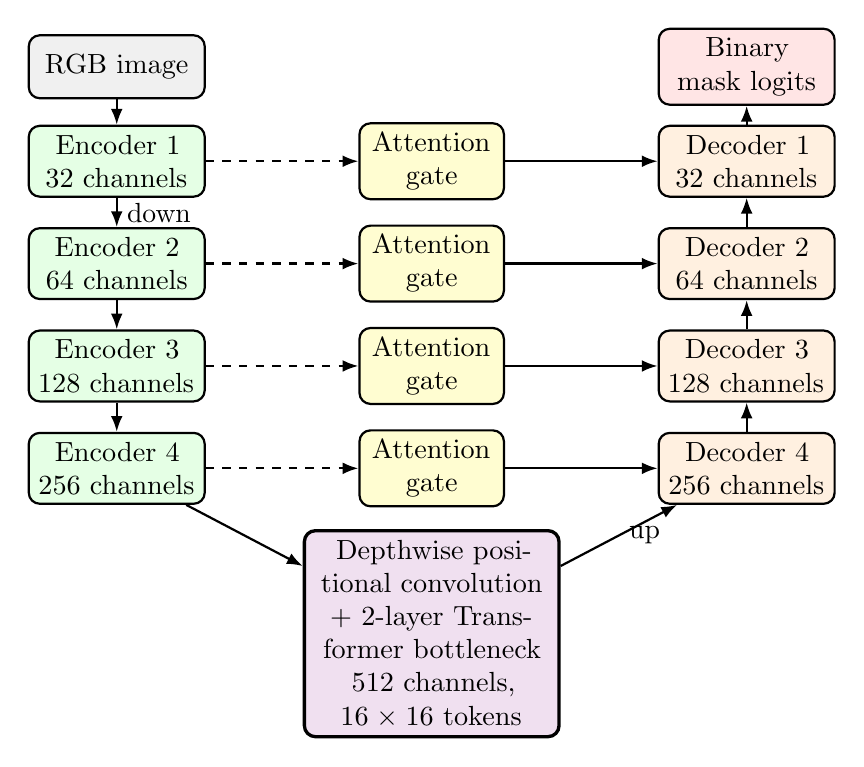
\begin{tikzpicture}
  \node[block,fill=gray!12] (input) at (0,0) {RGB image};
  \node[enc] (e1) at (0,-1.2) {Encoder 1\\$32$ channels};
  \node[enc] (e2) at (0,-2.5) {Encoder 2\\$64$ channels};
  \node[enc] (e3) at (0,-3.8) {Encoder 3\\$128$ channels};
  \node[enc] (e4) at (0,-5.1) {Encoder 4\\$256$ channels};
  \node[trans] (t) at (4,-7.2) {Depthwise positional convolution\\+ 2-layer Transformer bottleneck\\$512$ channels, $16\times16$ tokens};
  \node[dec] (d4) at (8,-5.1) {Decoder 4\\$256$ channels};
  \node[dec] (d3) at (8,-3.8) {Decoder 3\\$128$ channels};
  \node[dec] (d2) at (8,-2.5) {Decoder 2\\$64$ channels};
  \node[dec] (d1) at (8,-1.2) {Decoder 1\\$32$ channels};
  \node[block,fill=red!10] (out) at (8,0) {Binary mask logits};

  \draw[flow] (input)--(e1);
  \draw[flow] (e1)--node[right]{down}(e2);
  \draw[flow] (e2)--(e3);
  \draw[flow] (e3)--(e4);
  \draw[flow] (e4)--(t);
  \draw[flow] (t)--node[right]{up}(d4);
  \draw[flow] (d4)--(d3);
  \draw[flow] (d3)--(d2);
  \draw[flow] (d2)--(d1);
  \draw[flow] (d1)--(out);

  \node[att] (a1) at (4,-1.2) {Attention\\gate};
  \node[att] (a2) at (4,-2.5) {Attention\\gate};
  \node[att] (a3) at (4,-3.8) {Attention\\gate};
  \node[att] (a4) at (4,-5.1) {Attention\\gate};
  \draw[skip] (e1)--(a1); \draw[flow] (a1)--(d1);
  \draw[skip] (e2)--(a2); \draw[flow] (a2)--(d2);
  \draw[skip] (e3)--(a3); \draw[flow] (a3)--(d3);
  \draw[skip] (e4)--(a4); \draw[flow] (a4)--(d4);
\end{tikzpicture}%
}
\caption{Full attention-plus-Transformer U-Net variant. The four experiments use the same encoder-decoder; attention gates and the Transformer bottleneck are enabled or disabled to form the controlled ablations.}
\label{fig:architecture}
\end{figure}
\FloatBarrier

For encoder skip $x$ and decoder gating feature $g$, the attention coefficient is
\begin{equation}
\alpha=\sigma\left(\psi^{\top}\operatorname{ReLU}(W_xx+W_gg+b)\right),
\qquad \tilde{x}=\alpha\odot x.
\end{equation}
The filtered skip $\tilde{x}$ is concatenated with the upsampled decoder feature. The Transformer bottleneck first adds a depthwise-convolution positional residual, flattens the feature map into tokens, and applies two encoder layers with eight heads. Because attention is used only at $1/16$ input resolution, token count and memory remain much lower than full-resolution attention.

\subsection{Training Objective}

The loss combines binary cross-entropy and soft Dice loss:
\begin{equation}
\mathcal{L}=0.5\mathcal{L}_{\mathrm{BCE}}+0.5\mathcal{L}_{\mathrm{Dice}},
\end{equation}
where
\begin{equation}
\mathcal{L}_{\mathrm{Dice}}=1-\frac{2\sum_i p_i y_i+\epsilon}{\sum_i p_i^2+\sum_i y_i^2+\epsilon}.
\end{equation}
BCE supplies pixel-wise supervision, while Dice directly addresses foreground-background imbalance.

\FloatBarrier
\Needspace{6\baselineskip}
\section{Experimental Setup}
\label{sec:experiments}

\subsection{Data Split and Preprocessing}

The 1,000 Kvasir-SEG pairs are deterministically shuffled with seed 42 and divided into 700 training, 150 validation, and 150 testing images. The split is stored as a CSV file and reused unchanged by every experiment. Images and masks are resized to $256\times256$. Training augmentation includes horizontal flipping, occasional vertical flipping, rotation up to $20^{\circ}$, and random brightness/contrast adjustment. Validation and test images are resized and normalized without stochastic augmentation.

The use of one fixed split supports controlled ablation but does not measure split variability. A stronger future study should repeat the experiment with multiple seeds or cross-validation.

\begin{figure}[H]
\centering
\resizebox{0.98\textwidth}{!}{%
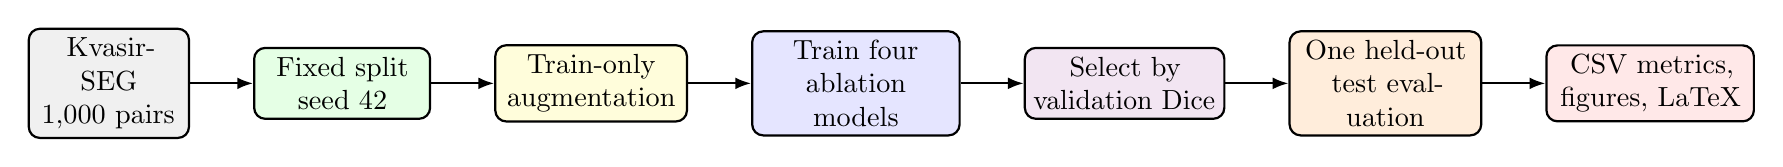
\begin{tikzpicture}[node distance=8mm]
  \node[block,fill=gray!12,text width=18mm] (data) {Kvasir-SEG\\1,000 pairs};
  \node[block,fill=green!10,text width=20mm,right=of data] (split) {Fixed split\\seed 42};
  \node[block,fill=yellow!14,text width=22mm,right=of split] (aug) {Train-only\\augmentation};
  \node[block,fill=blue!10,text width=24mm,right=of aug] (train) {Train four\\ablation models};
  \node[block,fill=violet!10,text width=23mm,right=of train] (select) {Select by\\validation Dice};
  \node[block,fill=orange!14,text width=22mm,right=of select] (test) {One held-out\\test evaluation};
  \node[block,fill=red!9,text width=24mm,right=of test] (report) {CSV metrics,\\figures, LaTeX};
  \draw[flow] (data)--(split);
  \draw[flow] (split)--(aug);
  \draw[flow] (aug)--(train);
  \draw[flow] (train)--(select);
  \draw[flow] (select)--(test);
  \draw[flow] (test)--(report);
\end{tikzpicture}%
}
\caption{Experimental workflow. The test set is isolated until final evaluation, and all reported tables and figures are generated from saved machine-readable results.}
\label{fig:workflow}
\end{figure}
\FloatBarrier

\subsection{Compared Configurations}

\begin{table}[H]
\centering
\caption{Controlled architectural ablation.}
\label{tab:ablation-design}
\begin{tabular}{lcc}
\toprule
\textbf{Configuration} & \textbf{Attention skips} & \textbf{Transformer bottleneck}\\
\midrule
U-Net & No & No\\
Attention U-Net & Yes & No\\
Transformer U-Net & No & Yes\\
Attention + Transformer & Yes & Yes\\
\bottomrule
\end{tabular}
\end{table}

All configurations use base width 32, four downsampling stages, batch size 4, 30 maximum epochs, AdamW with learning rate $10^{-4}$ and weight decay $10^{-4}$ \cite{loshchilov2019adamw}, cosine learning-rate decay, mixed precision when CUDA is available, and early stopping after seven validation epochs without Dice improvement. The checkpoint with the highest validation Dice is evaluated once on the held-out test set.

\subsection{Implementation and Computational Protocol}

The experiments are implemented in PyTorch and executed on \HardwareName~using PyTorch \TorchVersion, CUDA \CudaVersion, and Python \PythonVersion. Final evaluation was performed on \EvaluationDate. These values are generated from the evaluation logs rather than typed manually. Convolutional layers use batch normalization and ReLU activation, while the Transformer encoder uses pre-normalization, GELU feed-forward activation, residual connections, and dropout 0.1. The bottleneck contains 512 channels and eight attention heads, so each head receives a 64-dimensional representation. At the $16\times16$ bottleneck resolution, the token sequence contains 256 elements. This design limits the quadratic attention matrix to $256\times256$, which is substantially smaller than applying attention to all $256\times256$ input pixels.

Training uses automatic mixed precision on CUDA to reduce memory use and accelerate compatible operations. Gradients are reset with \texttt{set\_to\_none=True}, and the best checkpoint is selected exclusively using validation Dice. Inference latency is measured after warm-up iterations, synchronized on CUDA, and divided by both the number of timed iterations and batch size. Parameter count includes all model parameters, while trainable parameter count is also stored in the JSON output. Because latency varies with hardware and software, the paper reports the exact device and treats timing as an implementation-specific efficiency measurement rather than a universal property of the architecture.

\subsection{Leakage Prevention and Experimental Integrity}

The test set is not used for early stopping, threshold tuning, architecture selection, or data augmentation decisions. A single CSV split is generated before model training and reused by all configurations, which prevents accidental differences in sample composition. Augmentation is applied only to the training subset. Validation and test transformations contain deterministic resizing and normalization. Each checkpoint stores the full configuration together with the model state, selected epoch, optimizer state, and best validation Dice, making it possible to verify which settings produced a reported result.

The result pipeline also separates measurement from reporting. The evaluation script writes per-image metrics and aggregate statistics to machine-readable files. The paper values are then generated from those files through \texttt{generate\_paper\_assets.py}. This reduces the risk of copying a value from the wrong run, rounding inconsistently, or mixing validation and test results. The repository intentionally retains the raw histories and summaries but excludes the dataset and large checkpoints from normal version control.

\subsection{Hyperparameter Rationale}

The image size of 256 was selected as a compromise between preserving polyp boundaries and fitting all configurations on a consumer GPU. The base width of 32 keeps the convolutional baseline sufficiently expressive while leaving memory for the Transformer ablations. Batch size 4 is used unchanged across models so that optimization noise and batch-normalization behavior remain comparable. The learning rate $10^{-4}$ is conservative for training from scratch with AdamW, while cosine decay gradually reduces the update magnitude without requiring model-specific milestone selection. The equal BCE and Dice weights balance pixel-wise calibration with overlap optimization. Early stopping limits overfitting and avoids choosing a fixed epoch that may favor one architecture. No architecture-specific learning rate, augmentation, threshold, or training duration is introduced, because such tuning would weaken the interpretation of the ablation. These settings are not claimed to be globally optimal; rather, they define a transparent common operating point suitable for testing the two architectural hypotheses under limited time and computation.

\subsection{Evaluation Metrics}

Dice and IoU measure region overlap:
\begin{equation}
\mathrm{Dice}=\frac{2TP}{2TP+FP+FN},\qquad
\mathrm{IoU}=\frac{TP}{TP+FP+FN}.
\end{equation}
Precision measures false-positive control, while recall measures the proportion of polyp pixels recovered. HD95 measures the 95th percentile of bidirectional boundary distances and captures contour errors not visible in overlap alone \cite{taha2015metrics}. HD95 is reported in pixels after resizing, so it should not be interpreted as a physical clinical distance. Efficiency is evaluated using parameter count and average inference milliseconds per image on the recorded device.

\subsection{Reproducibility}

The implementation fixes Python, NumPy, and PyTorch random seeds and requests deterministic algorithms where supported. Every run saves configuration, best and last checkpoints, per-epoch history, per-image test metrics, aggregate JSON metrics, and hardware information. The paper imports automatically generated LaTeX macros from the evaluation output, reducing manual transcription errors. The public repository is \url{https://github.com/hammiroussama/lightweight-transformer-unet-kvasir}.

\FloatBarrier
\Needspace{6\baselineskip}
\section{Results}
\label{sec:results}

\subsection{Main Quantitative Results}

\begin{table}[H]
\centering
\caption{Test-set results under the identical protocol. HD95 is measured in resized-image pixels. Lower HD95 is better; higher values are better for all other accuracy metrics.}
\label{tab:main-results}
\scriptsize
\begin{tabular}{lrrrrrrr}
\toprule
\textbf{Model} & \textbf{Dice} & \textbf{IoU} & \textbf{Precision} & \textbf{Recall} & \textbf{HD95} & \textbf{Parameters} & \textbf{ms/image}\\
\midrule
U-Net & \UNetDice & \UNetIoU & \UNetPrecision & \UNetRecall & \UNetHD & \textbf{\UNetParams} & \textbf{\UNetLatency}\\
Attention U-Net & \AttentionUNetDice & \AttentionUNetIoU & \AttentionUNetPrecision & \AttentionUNetRecall & \AttentionUNetHD & \AttentionUNetParams & \AttentionUNetLatency\\
Transformer U-Net & \textbf{\TransformerUNetDice} & \textbf{\TransformerUNetIoU} & \textbf{\TransformerUNetPrecision} & \TransformerUNetRecall & \textbf{\TransformerUNetHD} & \TransformerUNetParams & \TransformerUNetLatency\\
Proposed (Attention + Transformer) & \ProposedDice & \ProposedIoU & \ProposedPrecision & \textbf{\ProposedRecall} & \ProposedHD & \ProposedParams & \ProposedLatency\\
\bottomrule
\end{tabular}
\end{table}
\FloatBarrier

Transformer U-Net achieved the best overall result, with Dice \TransformerUNetDice, IoU \TransformerUNetIoU, precision \TransformerUNetPrecision, and HD95 \TransformerUNetHD~pixels. Relative to U-Net, its Dice increased by \DiceGain~(8.87 percentage points), while HD95 decreased by 20.42 pixels, or approximately 40.8\%. Attention U-Net also improved the baseline, increasing Dice from \UNetDice~to \AttentionUNetDice~with only a small parameter increase. The attention-plus-Transformer model obtained the highest recall (\ProposedRecall), but its Dice and IoU were slightly lower than Transformer U-Net and its latency increased to \ProposedLatency~ms per image. Therefore, the two components were not fully complementary under the tested protocol. Table~\ref{tab:main-results} should be interpreted as a controlled single-seed ablation rather than a state-of-the-art benchmark comparison. The per-image Dice standard deviations were 0.2400, 0.2049, 0.1870, and 0.1807 for U-Net, Attention U-Net, Transformer U-Net, and the proposed model, respectively. These values describe variation across the 150 test images and must not be interpreted as run-to-run uncertainty.

\IfFileExists{figures/test_dice_comparison.png}{
\begin{figure}[H]
\centering
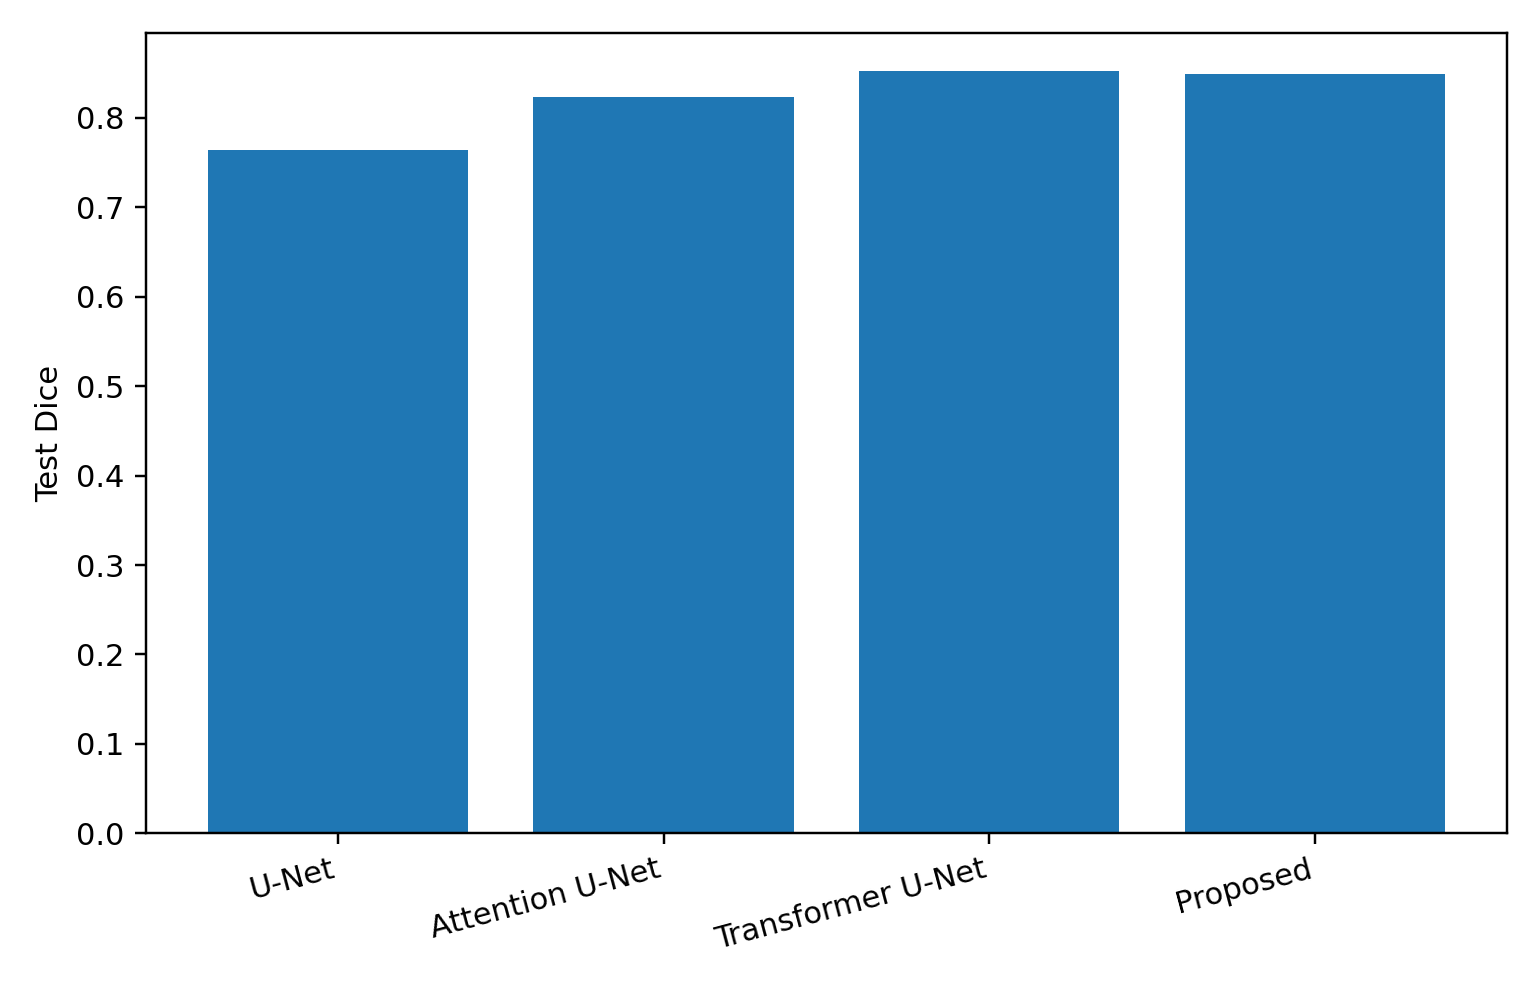
\includegraphics[width=0.72\textwidth]{figures/test_dice_comparison.png}
\caption{Test Dice comparison generated directly from the experiment summaries.}
\label{fig:test-dice}
\end{figure}
}{\begin{figure}[H]\centering\fbox{\parbox{0.75\textwidth}{Run \texttt{python run\_all\_experiments.py} to generate the test Dice comparison.}}\caption{Placeholder for the automatically generated test Dice figure.}\end{figure}}
\FloatBarrier

\Needspace{0.60\textheight}
\subsection{Training Behavior}

The validation curves document the optimization trajectories and the epochs used for checkpoint selection. U-Net stopped earlier than the other variants, whereas the Transformer-based models continued improving through later epochs. The combined model reached the highest late validation Dice, but Transformer U-Net obtained the best held-out test Dice. This validation--test ranking difference illustrates why architecture selection should be based on a fixed validation protocol while final claims must be made from the untouched test set. Because only one training run was performed for each configuration, minor differences in curve smoothness should not be interpreted as evidence of architectural superiority. Figure~\ref{fig:curves} presents the complete validation trajectories without interrupting this analysis.

\IfFileExists{figures/validation_dice_curves.png}{
\begin{figure}[H]
\centering
\begin{minipage}{0.48\textwidth}\centering
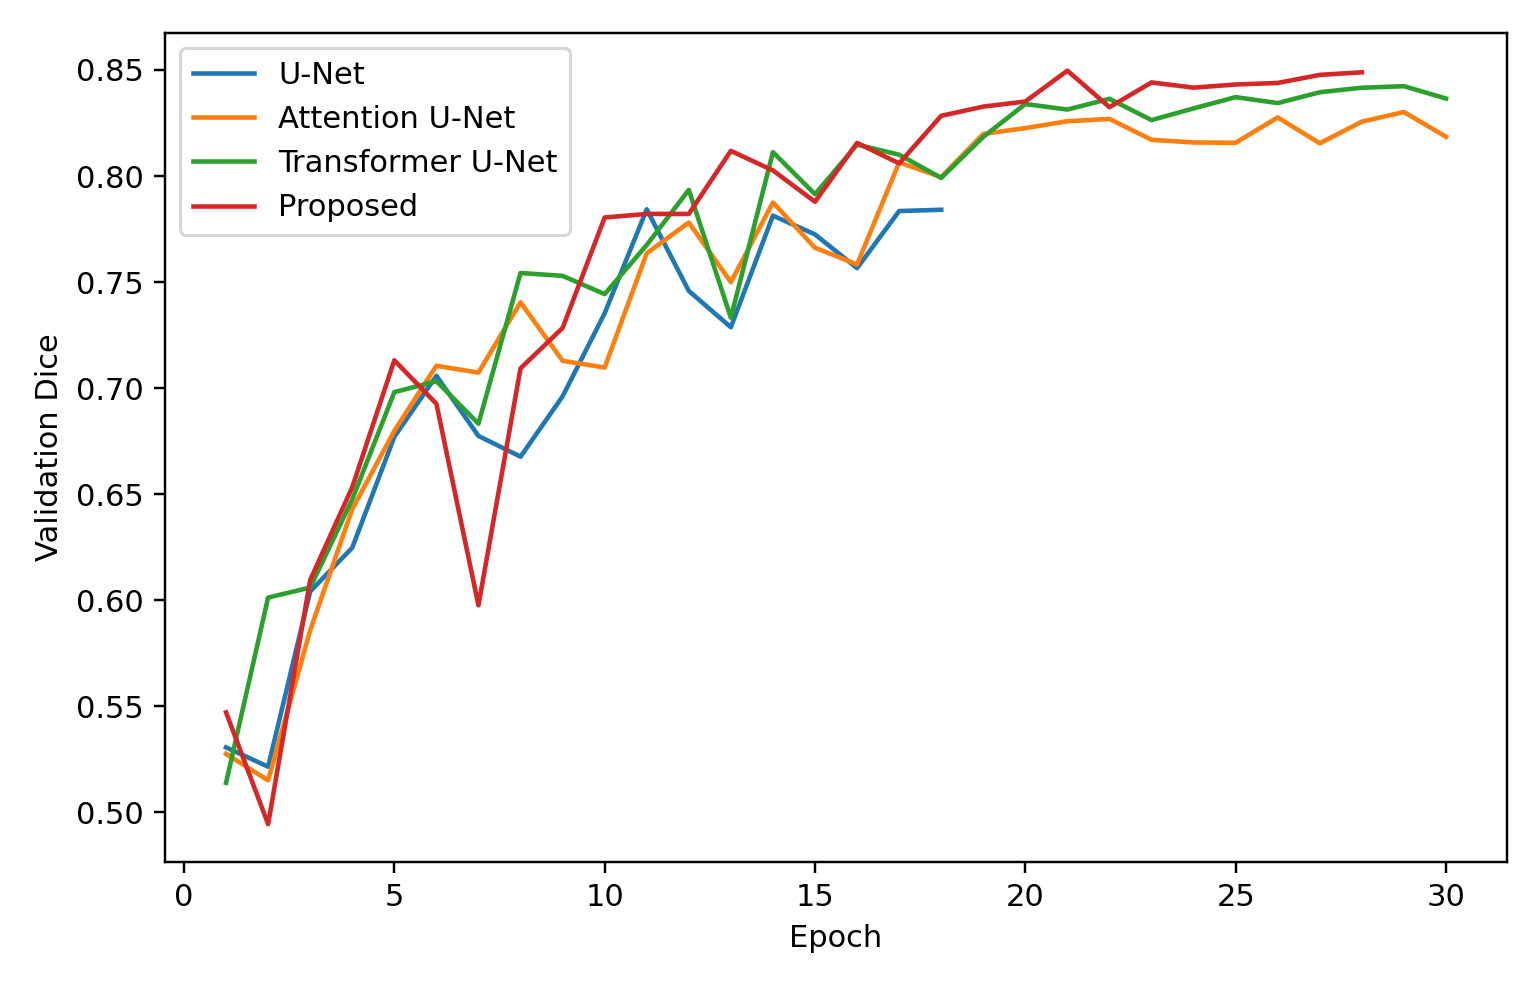
\includegraphics[width=\linewidth]{figures/validation_dice_curves.png}
\end{minipage}\hfill
\begin{minipage}{0.48\textwidth}\centering
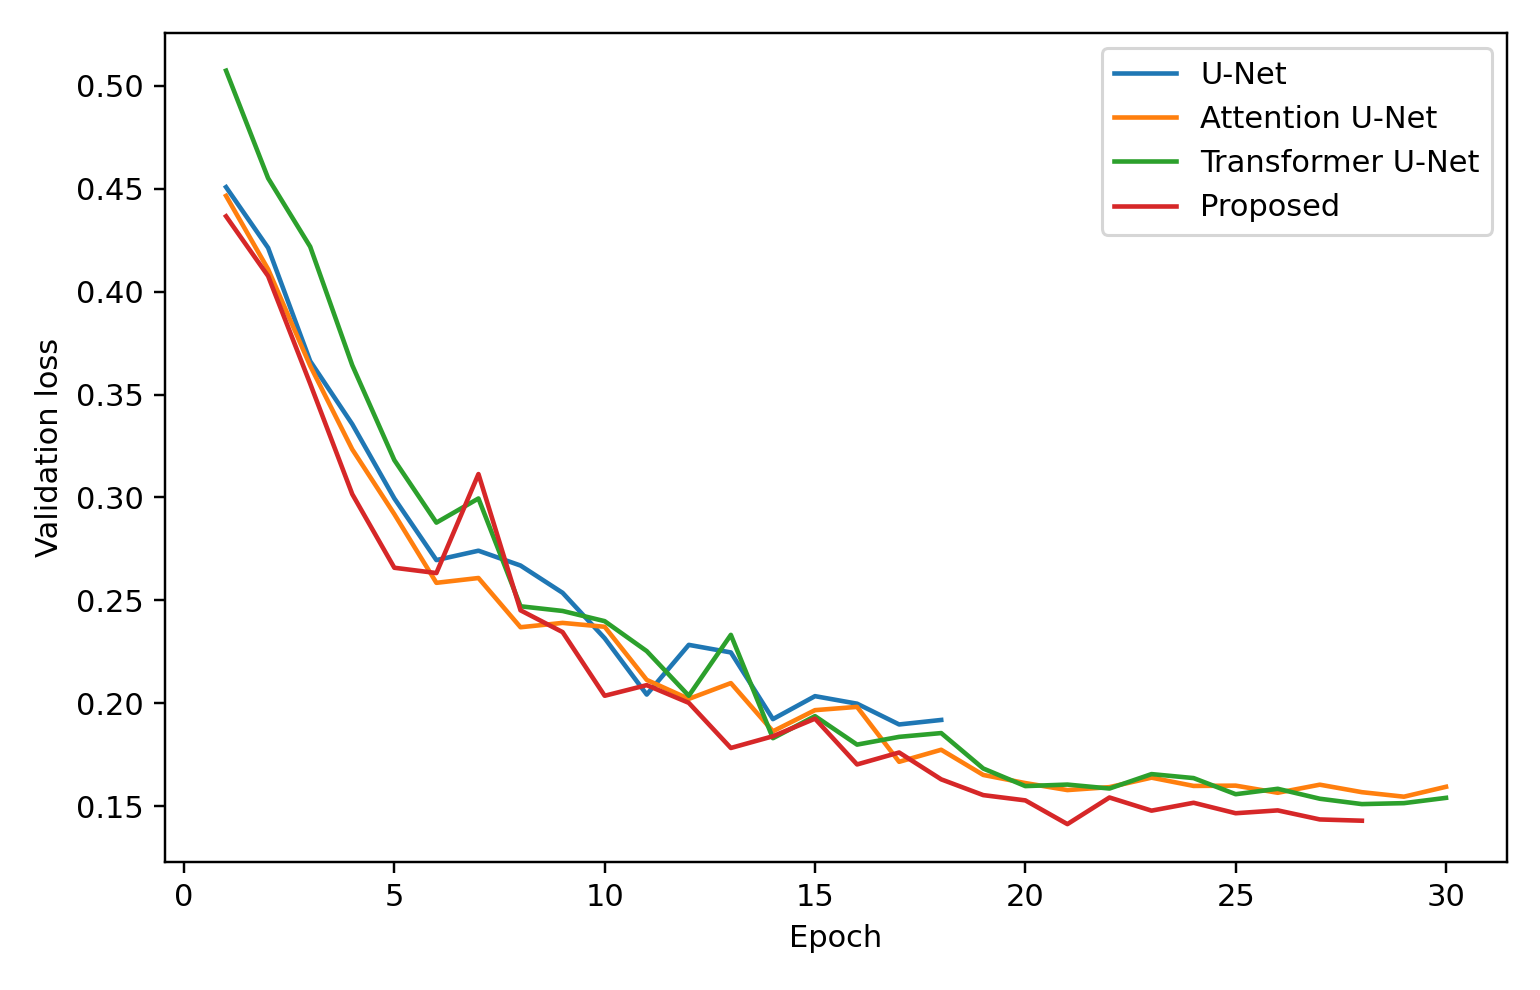
\includegraphics[width=\linewidth]{figures/validation_loss_curves.png}
\end{minipage}
\caption{Validation Dice and loss curves generated from the saved training histories. The curves document convergence and the checkpoint-selection process.}
\label{fig:curves}
\end{figure}
}{\begin{figure}[H]\centering\fbox{\parbox{0.75\textwidth}{Training curves are generated after all experiments finish.}}\caption{Placeholder for validation curves.}\end{figure}}
\FloatBarrier

\Needspace{0.72\textheight}
\subsection{Qualitative Analysis}

Figure~\ref{fig:qualitative} includes both difficult and successful test examples rather than only favorable cases. The examples were selected automatically using the recorded per-image metrics, so the visual comparison complements rather than replaces the aggregate evaluation.

\IfFileExists{figures/qualitative_results.png}{
\begin{figure}[H]
\centering
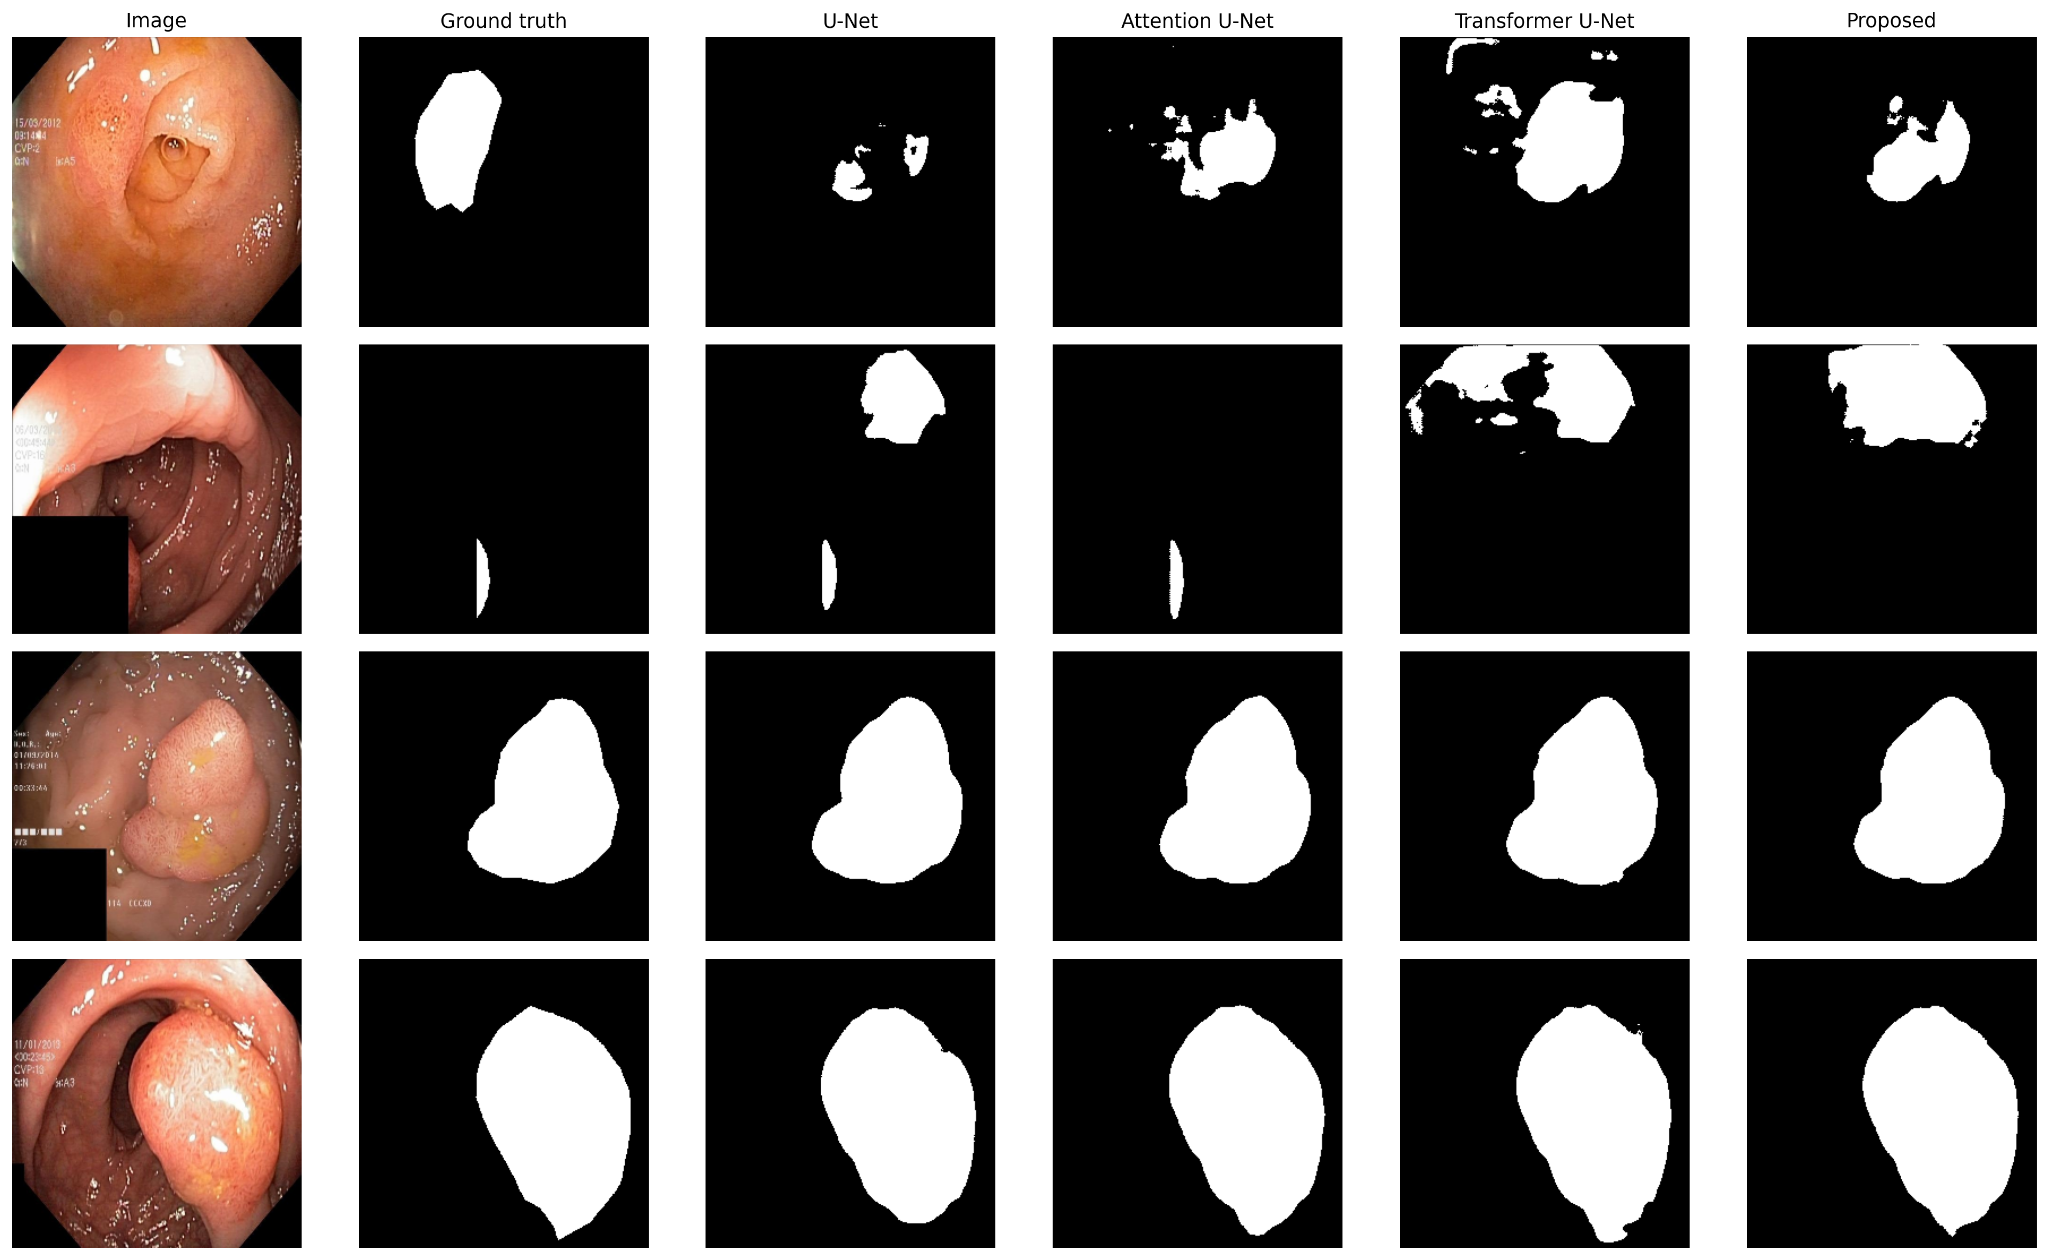
\includegraphics[width=0.98\textwidth]{figures/qualitative_results.png}
\caption{Qualitative comparison on automatically selected difficult and strong test cases. The sample names and selection rule are recorded in \texttt{results/qualitative\_samples.csv}. The figure must be interpreted together with quantitative metrics because visually plausible masks may still contain clinically relevant boundary errors.}
\label{fig:qualitative}
\end{figure}
}{\begin{figure}[H]\centering\fbox{\parbox{0.75\textwidth}{Qualitative predictions are generated after all four checkpoints are evaluated.}}\caption{Placeholder for image, ground-truth, and four-model prediction comparisons.}\end{figure}}

In the first difficult example, U-Net severely under-segments the target, whereas the attention-based variants recover a larger portion of the polyp; Transformer U-Net also produces disconnected false-positive regions. In the second difficult example, U-Net and Attention U-Net identify the small target, while both Transformer-containing models over-segment a large upper region. By contrast, the third and fourth examples show close agreement among all models for large, high-contrast polyps, with only small boundary differences. These observations explain why average Dice improves with contextual modeling while individual cases can still fail because of specular highlights, low contrast, or misleading global appearance. Qualitative examples support error analysis but do not replace aggregate test metrics.
\FloatBarrier
\Needspace{6\baselineskip}
\section{Discussion}
\label{sec:discussion}

\subsection{In-Depth Interpretation Through Course Modules}

The controlled comparison provides three main findings. First, attention-gated skips were useful: Attention U-Net improved Dice by 5.96 percentage points and reduced HD95 from \UNetHD~to \AttentionUNetHD~pixels relative to U-Net, while adding only about 88 thousand parameters. From the visual-intelligence perspective, the gates act as learned feature selectors that reduce distracting shallow responses before decoder fusion.

Second, the Transformer bottleneck produced the largest overall improvement. Transformer U-Net increased Dice by 8.87 percentage points, increased recall from \UNetRecall~to \TransformerUNetRecall, and achieved the lowest HD95. This result illustrates a cross-module transfer from language intelligence to visual intelligence: self-attention supplies global content relationships that complement the local structural bias of convolution. Because self-attention was applied only to 256 bottleneck tokens, the improvement was obtained with moderate latency (\TransformerUNetLatency~ms per image) rather than the cost of full-resolution attention.

Third, combining both mechanisms did not yield the highest overlap accuracy. The attention-plus-Transformer model achieved the highest recall (\ProposedRecall), but it had lower precision, Dice, and IoU than Transformer U-Net and required \ProposedLatency~ms per image. A plausible interpretation is that the bottleneck already supplied sufficient contextual selectivity, so additional skip gating introduced redundancy or shifted the precision--recall balance. This explanation remains a hypothesis because the experiment uses one seed and does not include feature-level attribution.

\subsection{Research Advantages and Limitations}

The principal advantage is experimental control. All four configurations share the same split, preprocessing, augmentation, loss, optimizer, seed, checkpoint criterion, and test procedure, so the comparison isolates two architectural factors more clearly than an uncontrolled comparison of published scores. The study also combines overlap, boundary, classification-style, efficiency, convergence, and qualitative evidence, while the public repository exposes the complete implementation and machine-generated reporting pipeline.

Several limitations restrict the conclusions. Kvasir-SEG contains only 1,000 images from one application domain, one fixed split cannot measure split variability, and one random seed cannot quantify optimization uncertainty. Square resizing can distort aspect ratios and causes HD95 to be expressed in resized pixels. The experiment does not include external datasets, clinician assessment, repeated-seed statistical testing, or feature-attribution analysis. The lightweight bottleneck is also not a reproduction of a large pretrained TransUNet. Consequently, the results should be presented as a reproducible course experiment rather than clinical validation or a state-of-the-art claim \cite{maierhein2018rankings}.

\subsection{Course Learning Reflection}

Completing the project transformed several course concepts from isolated theory into one reproducible workflow. CNN encoder--decoder design clarified how structural intelligence supplies locality and hierarchical features; pixel-level masks and boundary metrics connected those representations to visual intelligence; and the Transformer bottleneck demonstrated how self-attention from language intelligence can be adapted to images. The most important practical challenge was not merely implementing a more complex model, but preserving a fair comparison. A deterministic split, shared configurations, validation-only checkpoint selection, and generated LaTeX macros were used to prevent leakage and reporting errors. Running the project on a shared GPU server and repairing Python-version and data-indexing issues also strengthened practical skills in environment management, debugging, and experiment traceability. The main lesson is that architectural novelty is meaningful only when supported by controlled variables, reliable measurements, and honest interpretation.

\subsection{Future Work Prospects}

The immediate priority is stronger visual-intelligence validation through three or more random seeds, cross-validation, and external datasets such as CVC-ClinicDB. Aspect-ratio-preserving preprocessing and calibrated uncertainty maps could improve boundary reliability. Generative intelligence may support carefully validated synthetic augmentation for rare polyp appearances, while multimodal intelligence could combine video frames, clinical metadata, or textual findings. An agent-intelligence extension could monitor uncertainty, identify suspicious failure cases, and request human correction instead of silently accepting an unreliable mask. These extensions should be evaluated incrementally so that their individual contributions remain identifiable rather than assuming that more modules automatically improve performance.

\subsection{Threats to Validity}

Several threats should be considered when interpreting the experiment. \textbf{Internal validity} concerns whether the observed differences are caused by the intended architectural changes. The shared split and training protocol reduce this threat, but stochastic optimization can still produce variation. One seed is sufficient for a time-limited course experiment but does not quantify run-to-run uncertainty. Repeating every configuration with at least three seeds and reporting mean, standard deviation, and paired per-image comparisons would strengthen the evidence.

\textbf{Construct validity} concerns whether the selected metrics represent the desired segmentation quality. Dice and IoU emphasize area overlap, precision and recall distinguish over- and under-segmentation, and HD95 measures boundary discrepancy. Nevertheless, these metrics do not directly measure whether segmentation improves polyp detection, clinician interpretation, or patient outcomes. HD95 is calculated after resizing and in pixel units, so it has no direct physical interpretation. Qualitative review is included to expose typical errors, but a clinician-rated evaluation would be stronger.

\textbf{External validity} concerns generalization beyond the study data. Kvasir-SEG represents one dataset and one type of endoscopic imagery. Performance may change with another hospital, endoscope manufacturer, bowel preparation quality, video compression, rare morphology, or external dataset. Resizing every image to a square may further change shape statistics. The current result should therefore be interpreted as evidence about the controlled Kvasir-SEG setting, not all colonoscopy environments.

\textbf{Conclusion validity} concerns whether the evidence is sufficient to support the stated conclusion. A small numerical difference may arise from random initialization or data ordering rather than a meaningful architectural advantage. The paper therefore avoids claiming superiority unless the difference is consistent across metrics, supported by qualitative behavior, and reasonable relative to parameter and latency cost. Future work should use repeated seeds, confidence intervals, bootstrapping of per-image metrics, and external testing.

\FloatBarrier
\Needspace{6\baselineskip}
\section{Code and Reproducibility}

All source code is publicly available in the \href{https://github.com/hammiroussama/lightweight-transformer-unet-kvasir}{project GitHub repository}. The repository contains model definitions, four fixed configurations, deterministic split generation, training and evaluation scripts, unit tests, result CSV files, generated figures, and scripts that transfer measured metrics into this paper. The dataset itself is not redistributed; users are directed to the official Kvasir-SEG source and must follow its research and educational terms.

A full reproduction is executed with:
\begin{verbatim}
python run_all_experiments.py
\end{verbatim}
The command trains all ablations, evaluates the selected checkpoints, writes the result tables, and creates the plotted paper figures. This automation is intended to prevent accidental mixing of results from different runs.

\FloatBarrier
\Needspace{6\baselineskip}
\section{Conclusion}
\label{sec:conclusion}

This paper investigated whether attention-gated skip connections and a lightweight Transformer bottleneck improve U-Net polyp segmentation under a controlled Kvasir-SEG protocol. The study connected three Advanced Artificial Intelligence course components: CNN-based structural intelligence, dense-prediction visual intelligence, and Transformer self-attention transferred from language intelligence. Four configurations were trained with the same split, preprocessing, augmentation, loss, optimizer, seed, checkpoint rule, and test procedure. Transformer U-Net achieved the strongest overall result, with Dice \TransformerUNetDice, IoU \TransformerUNetIoU, precision \TransformerUNetPrecision, and HD95 \TransformerUNetHD~pixels. Relative to U-Net, it improved Dice by \DiceGain~and reduced HD95 by approximately 40.8\%. Attention U-Net also improved the baseline with little parameter overhead. However, enabling both attention gates and the Transformer did not produce an additive gain: the combined model obtained the highest recall but lower Dice and IoU than Transformer U-Net and greater inference latency. The research question is therefore answered conditionally: both mechanisms can help U-Net, but global bottleneck context was the most valuable tested component, and extra complexity was not automatically beneficial. The conclusions remain limited by one dataset, one split, and one seed. The public GitHub repository provides code, configurations, measured results, generated figures, and the paper source for independent inspection and reproduction.

\appendix
\section{Reproducibility Pseudocode}
\label{app:pseudocode}

\begin{verbatim}
Input: Kvasir-SEG dataset D, fixed split S, configurations C
for each configuration c in C:
    set Python, NumPy, and PyTorch seed to 42
    train c only on S_train with train-only augmentation
    select checkpoint with maximum Dice on S_validation
    evaluate the selected checkpoint once on S_test
    save per-image metrics, aggregate metrics, and history
end for
generate comparison tables, figures, and LaTeX result macros
Output: reproducible CSV results, visualizations, and paper assets
\end{verbatim}

The executable implementation and exact configuration files are available at
\url{https://github.com/hammiroussama/lightweight-transformer-unet-kvasir}.

\bibliographystyle{IEEEtran}
\bibliography{references}

\end{document}
